\section{Common\-Emitter BJT Amplifier}

\subsection{Experiment Design}
    \subsubsection{Background}
    In this experiment, we want to measure the quiescent-point of a common-emitter BJT amplifier and evaluate the small-signal amplification function of a common-emitter amplifier.\par

    The Common\-Emitter have the property of high input impedence and high voltage gain.\par

    \subsubsection{Propose}
    \begin{itemize}
        \item To measure the quiescent-point of a common-emitter BJT amplifier
        \item To evaluate the small-signal amplification function of a common-emitter amplifier
    \end{itemize}

\subsection{Experiment Design}
    \subsubsection{Materials}
        In this experiment, we will use the following components:
        \begin{itemize}
            \item 2N3904\_1 BJT
            \item Resistors
            \item Capacitors
            \item DC power supply
            \item Digital Multi-Meter
            \item Function Generator
            \item Oscilloscope
        \end{itemize}

    \subsubsection{Circuit Diagram}
        The following circuit diagrams 
        \begin{figure}[H]
            \centering
            \includegraphics[width=0.5\linewidth]{Experiment_06/Circuit/Lab6.drawio.png}
            \caption{Common\-Emitter BJT Amplifier}
            \label{cir:6main}
        \end{figure}

    \subsubsection{Theoretical Analysis}
        \begin{enumerate}[I]
            \item \textbf{DC Analysis}
                First, we analyze the circuit by drawing its DC-equivalent circuit to find its quiescent working point.\par
                \begin{figure}[H]
                    \centering
                    \includegraphics[width=0.3\linewidth]{Experiment_06/Circuit/Lab6dc.drawio.png}
                    \caption{DC-equivalent Circuit}
                    \label{cir:6dc}
                \end{figure}
                In Fig.\ref{cir:6dc}, we can obtain the value of $R_{TH}$ and $V_{TH}$
                \begin{equation}
                    R_{\text{TH}} = R_a \parallel R_b, \quad V_{\text{TH}} = V \frac{R_b}{R_a + R_b}
                \end{equation}
                Then, we can calculate the value of $I_{\text{CQ}}$ and $V_{\text{CEQ}}$ by using the following equations:
                \begin{equation}
                    I_C = \beta I_B, \quad I_E = (1 + \beta) I_B, \quad V_C = 12 - I_C R_C, \quad V_B = V_{\text{TH}} - I_B R_B
                \end{equation}
                Finally, we can derive the value of $I_{\text{CQ}}$ and $V_{\text{CEQ}}$ by using the following equations:
                \begin{equation}
                    V_{\text{TH}} - I_B R_{\text{TH}} - V_{BE} - I_E R_E = 0, \quad I_B = \frac{V_{\text{TH}} - V_{BE}}{R_{\text{TH}} + (1+\beta)R_E}
                \end{equation}
            \item \textbf{AC Analysis}
                Next, we analyze the circuit by drawing its AC-equivalent circuit to find its small-signal amplification function.\par
                \begin{figure}[H]
                    \centering
                    \includegraphics[width=0.5\linewidth]{Experiment_06/Circuit/Lab6ac.drawio.png}
                    \caption{AC-equivalent Circuit}
                    \label{cir:6ac}
                \end{figure}
                In Fig.\ref{cir:6ac}, we can calculate the theoretical value of $V_O and V_i$, as well as the output and input impedence.
                \begin{equation*}
                    V_o = \beta i_B (R_C \parallel R_L)
                \end{equation*}
                \begin{equation*}
                    V_i = i_B r_\pi + \left(\frac{i_B r_\pi}{R_a} + \frac{i_B r_\pi}{R_b} + i_B \right) R_S
                \end{equation*}
                \begin{equation*}
                    R_i = R_a \parallel R_b \parallel r_\pi, 
                    \quad 
                    R_o = R_C \parallel R_L
                \end{equation*}
        \end{enumerate}

\subsection{Experiment record}
    \subsubsection{DC Analysis}
    Set $v_i$ euqals to zero, we can obtain the following data:
    \begin{table}[H]
        \centering
            \begin{tabular}{|l|ccccccc|}
            \hline
            & $V_B$ & $V_C$  & $V_E$ & $I_B$ & $I_C$  & $I_E$  & $\beta$ \\ \hline
            Meas & 3.776 & 10.435 & 3.118 & 12.3u & 1.565m & 1.553m & 127     \\ \hline
            Theo & 3.903 & 10.47  & 3     & 9.56u & 1.533m & 1.539m & 160     \\ \hline
        \end{tabular}
        \caption{Measured Data of DC Analysis}
        \end{table}
    From the table, we can see our theoretical data is close to the measured data, which means our theoretical analysis is correct.

    \subsubsection{AC Analysis}
    We adjust our $v_i$ in a rage that not distrot the output signal, and we can obtain the following data:
    \begin{table}[H]
        \centering
            \begin{tabular}{|l|cccc|}
            \hline
            $v_{ib}$ & 5.5  & 8.25 & 11   & 13.4 \\ \hline
            $v_o$    & 212  & 317  & 422  & 605  \\ \hline
            $A_v$    & 38.5 & 38.4 & 38.4 & 45.1 \\ \hline
        \end{tabular}
        \caption{Measured Data of AC Analysis}
    \end{table}

    And here is the plot output of the AC Analysis:
    \begin{figure}[H]
        \centering
        \begin{subfigure}{0.25\textwidth}
            \centering
            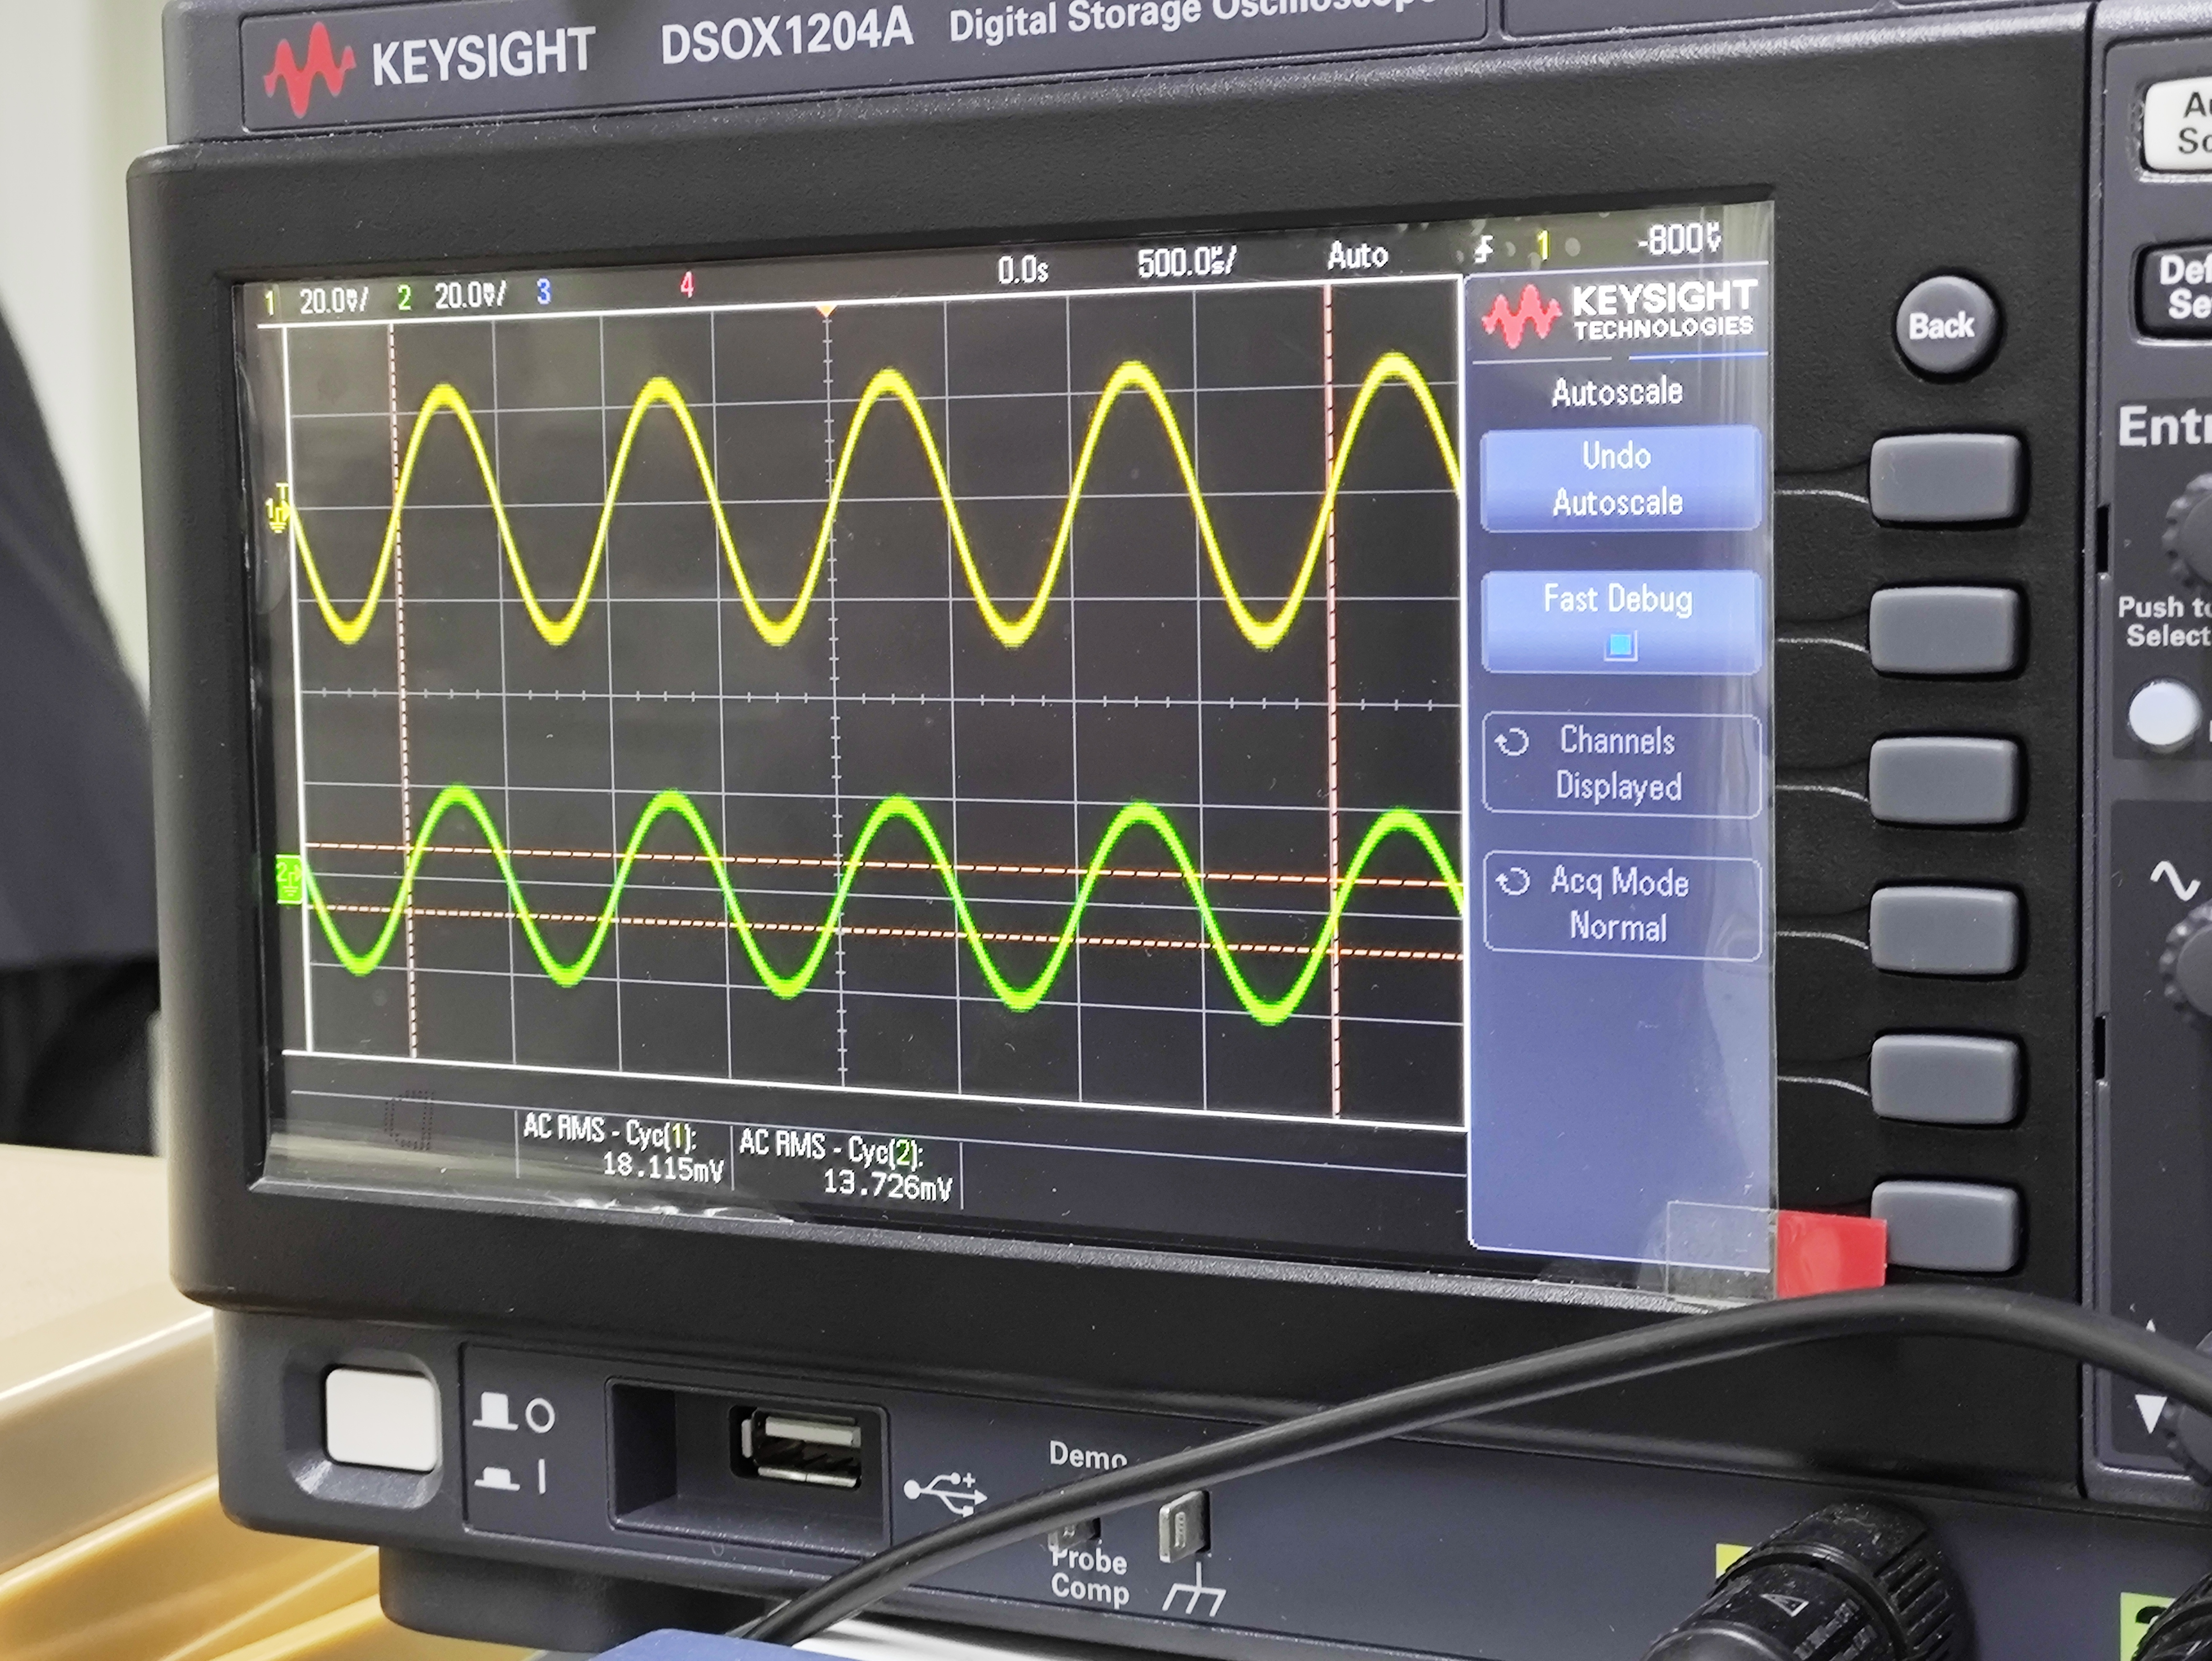
\includegraphics[width = 1\linewidth]{Experiment_06/Images/6.6_Vi-Vib_a.jpg}
            \caption{1000Hz, 0.5V peak}
            \label{l6acvg}
        \end{subfigure}
        \begin{subfigure}{0.25\textwidth}
            \centering
            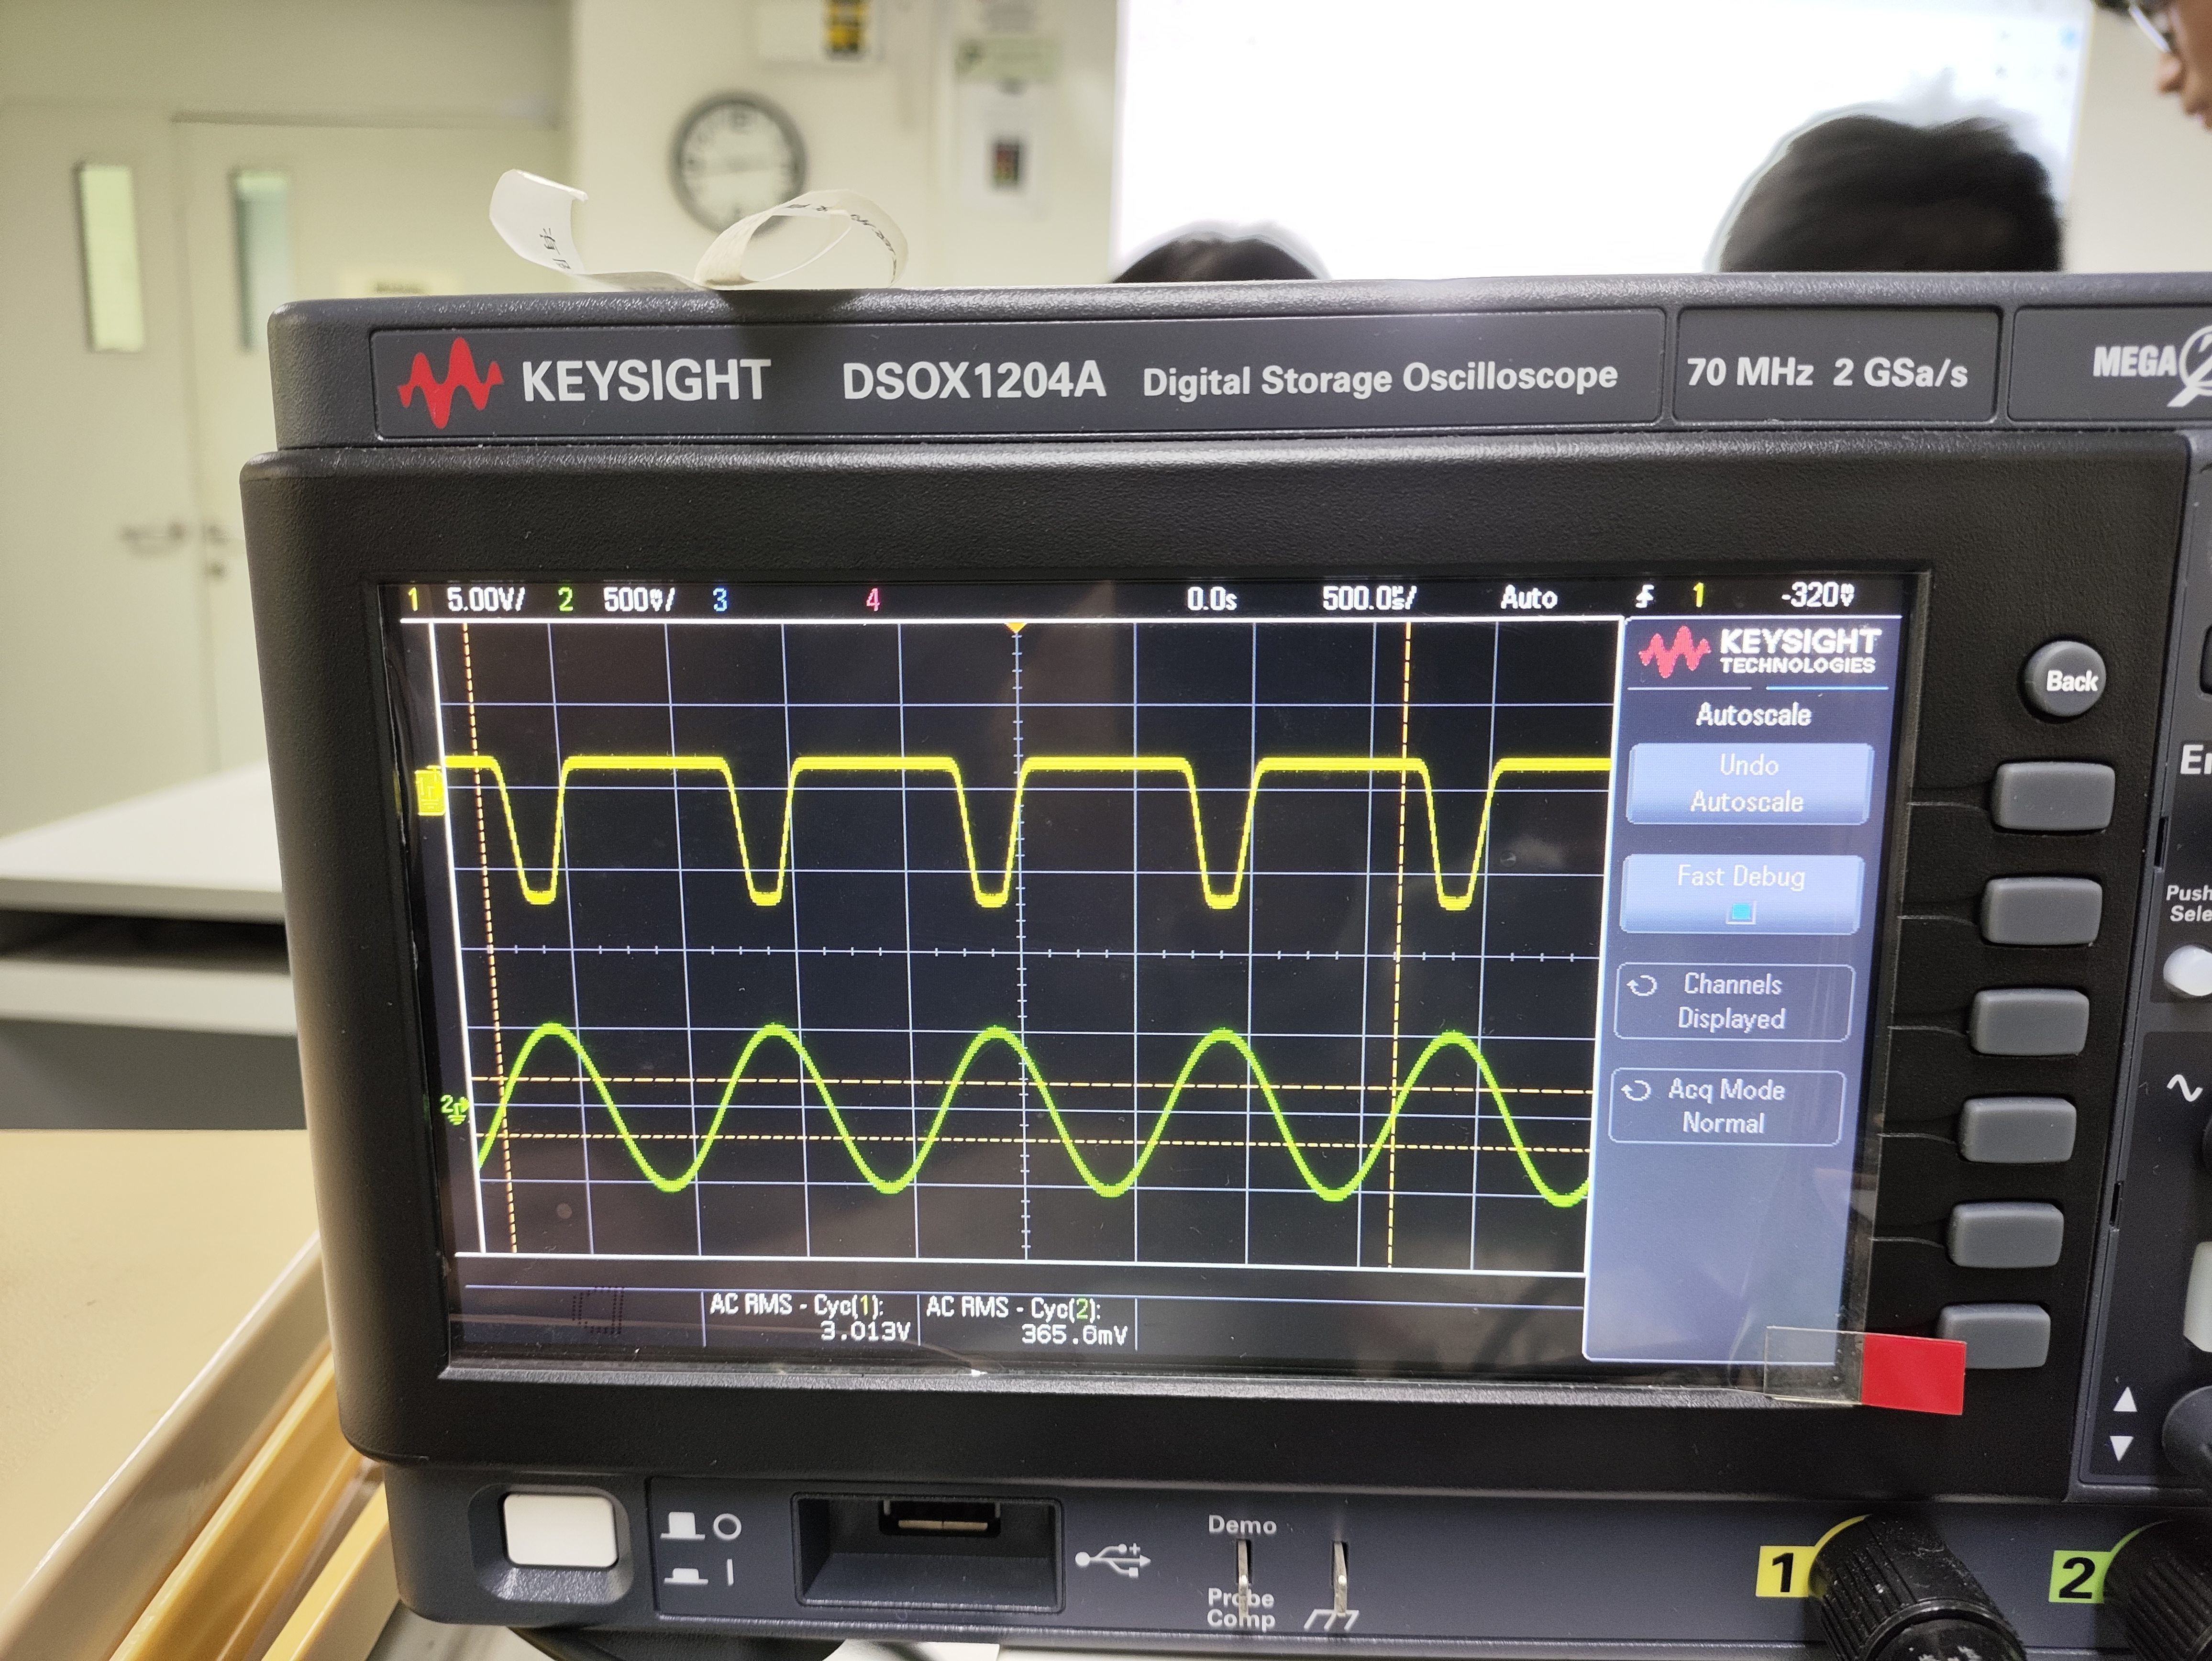
\includegraphics[width=1\linewidth]{Experiment_06/Images/6.5_Vo-Vib_distrupted.jpg}
            \caption{Disrupted Waveform}
            \label{l6dcdisrupted}
        \end{subfigure}
        \begin{subfigure}{0.25\textwidth}
            \centering
            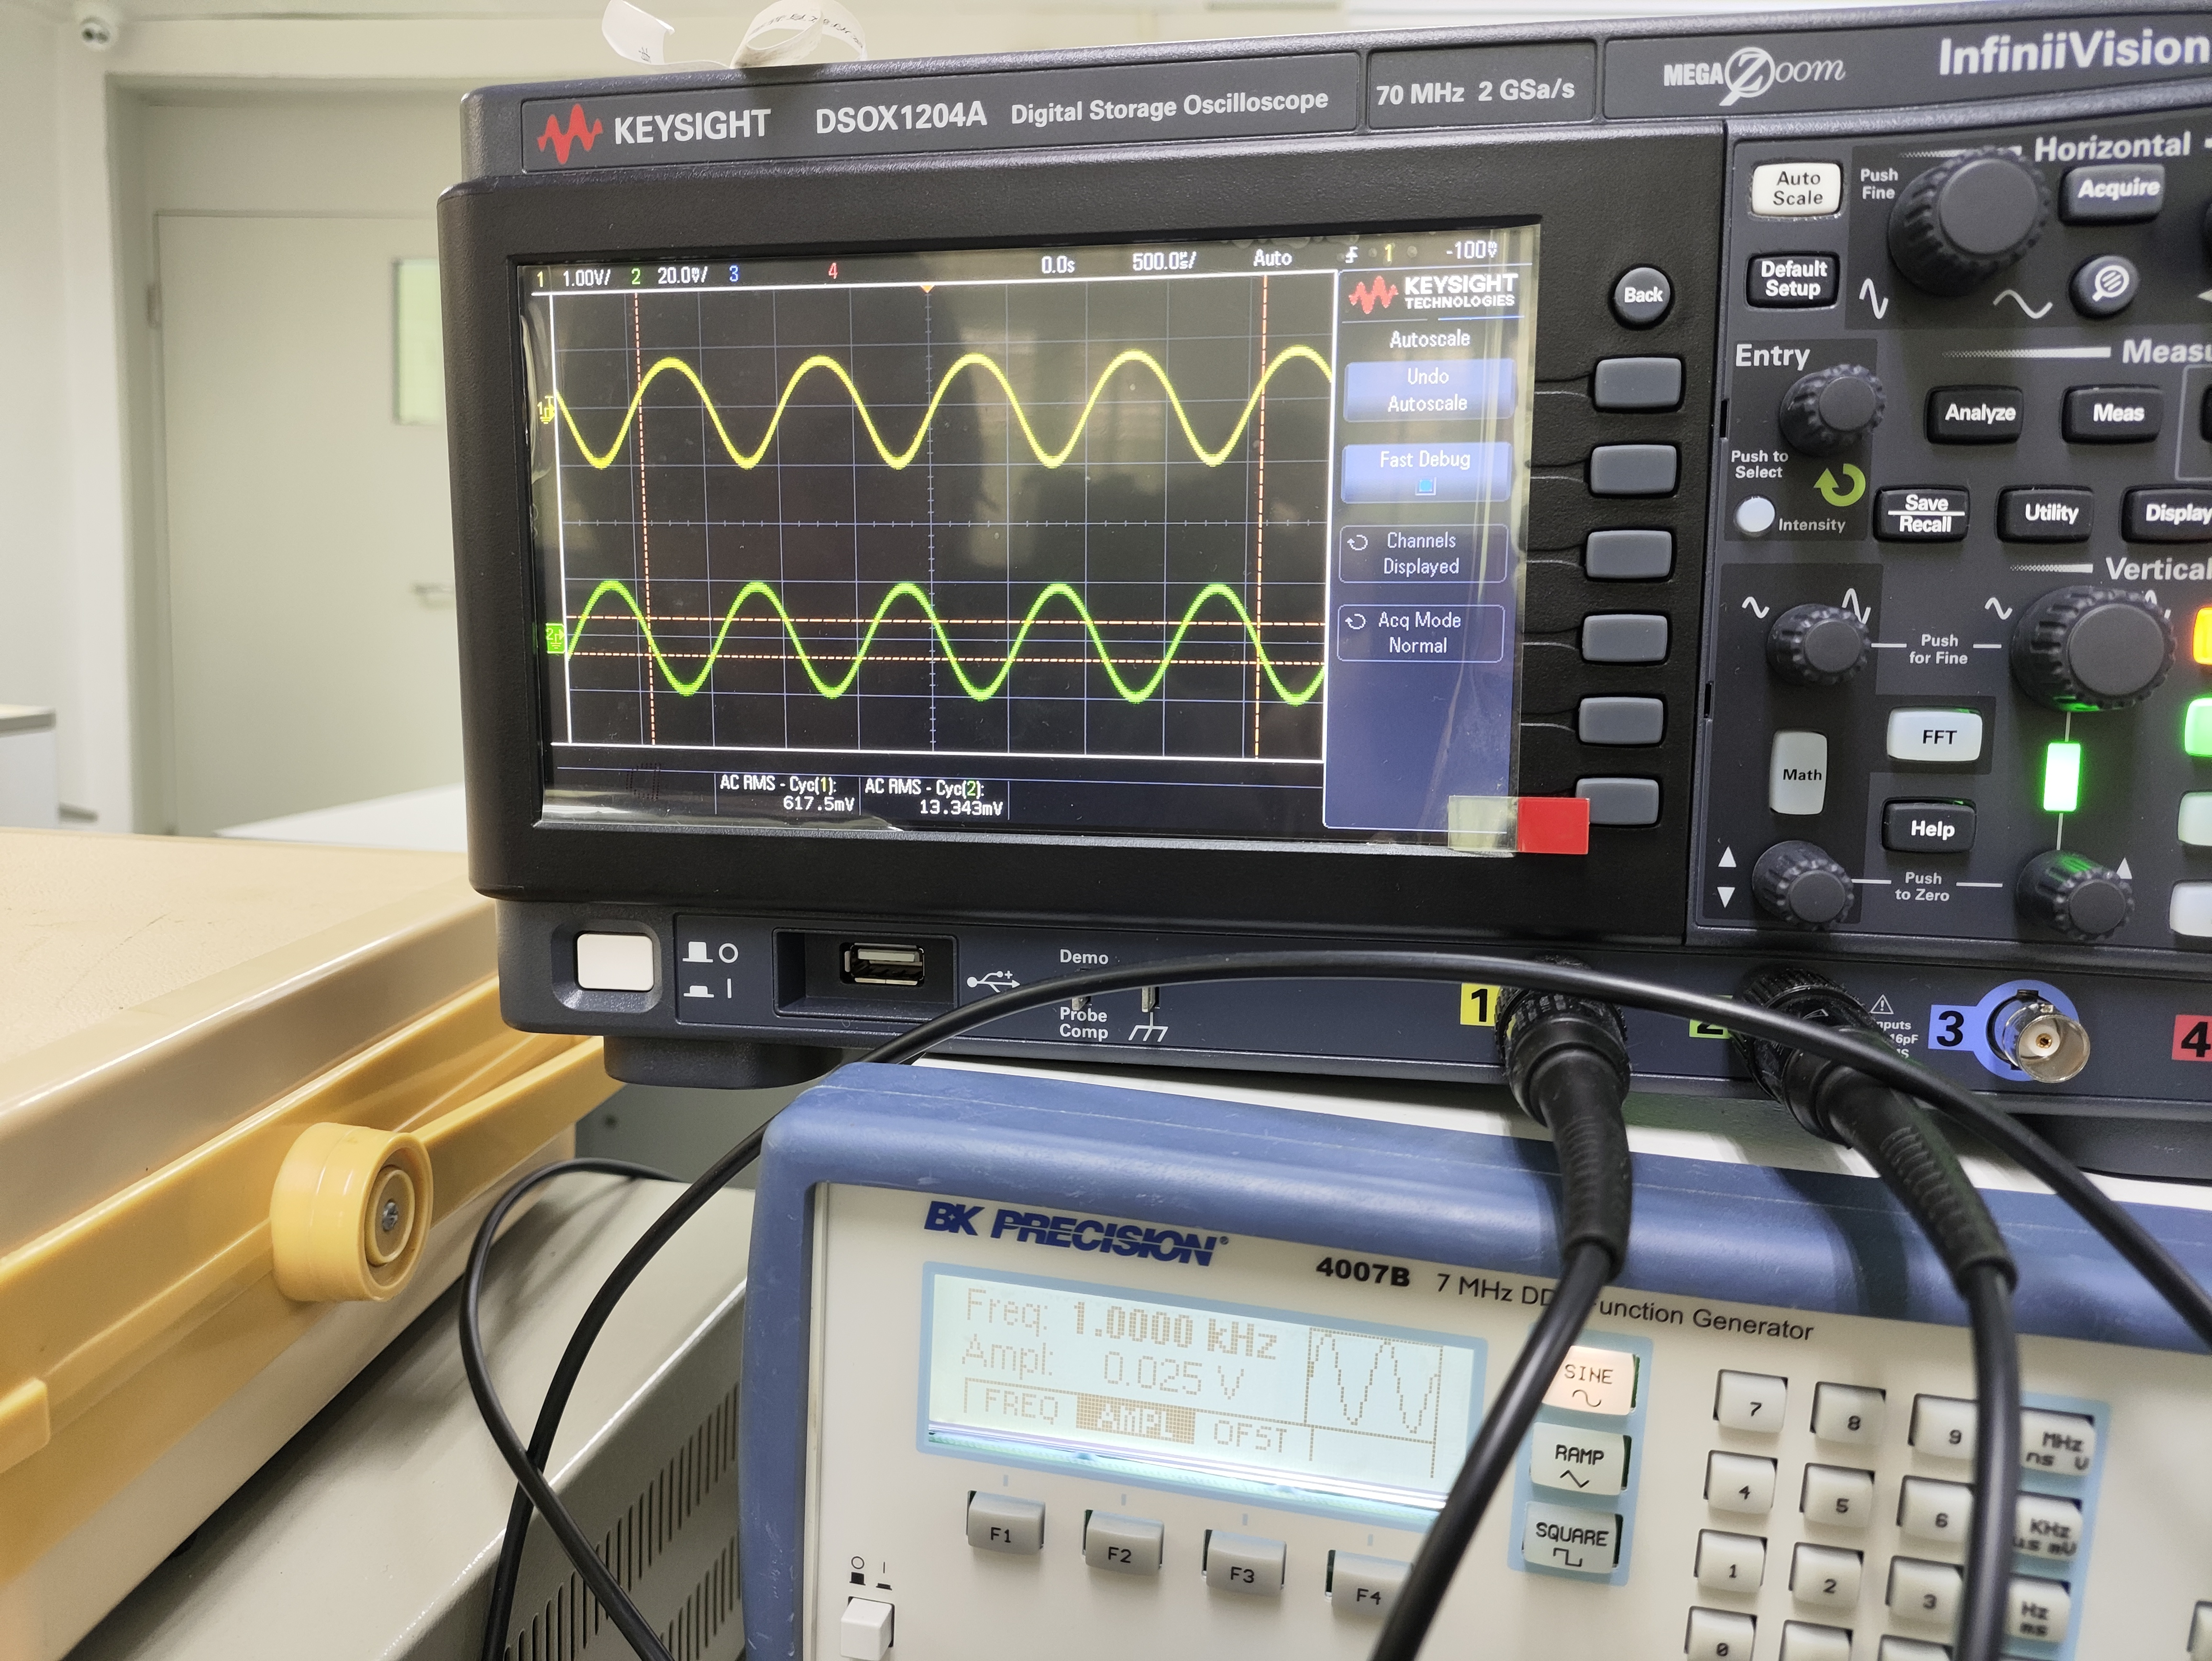
\includegraphics[width=1\linewidth]{Experiment_06/Images/6.5_Vo-Vib_025mV.jpg}
            \caption{0.025V Waveform}
            \label{l6dc025}
        \end{subfigure}

        \begin{subfigure}{0.25\textwidth}
            \centering
            \includegraphics[width=1\linewidth]{Experiment_06/Images/6.5_Vo-Vib_020mV.jpg}
            \caption{0.020V Waveform}
            \label{l6dc020}
        \end{subfigure}
        \begin{subfigure}{0.25\textwidth}
            \centering
            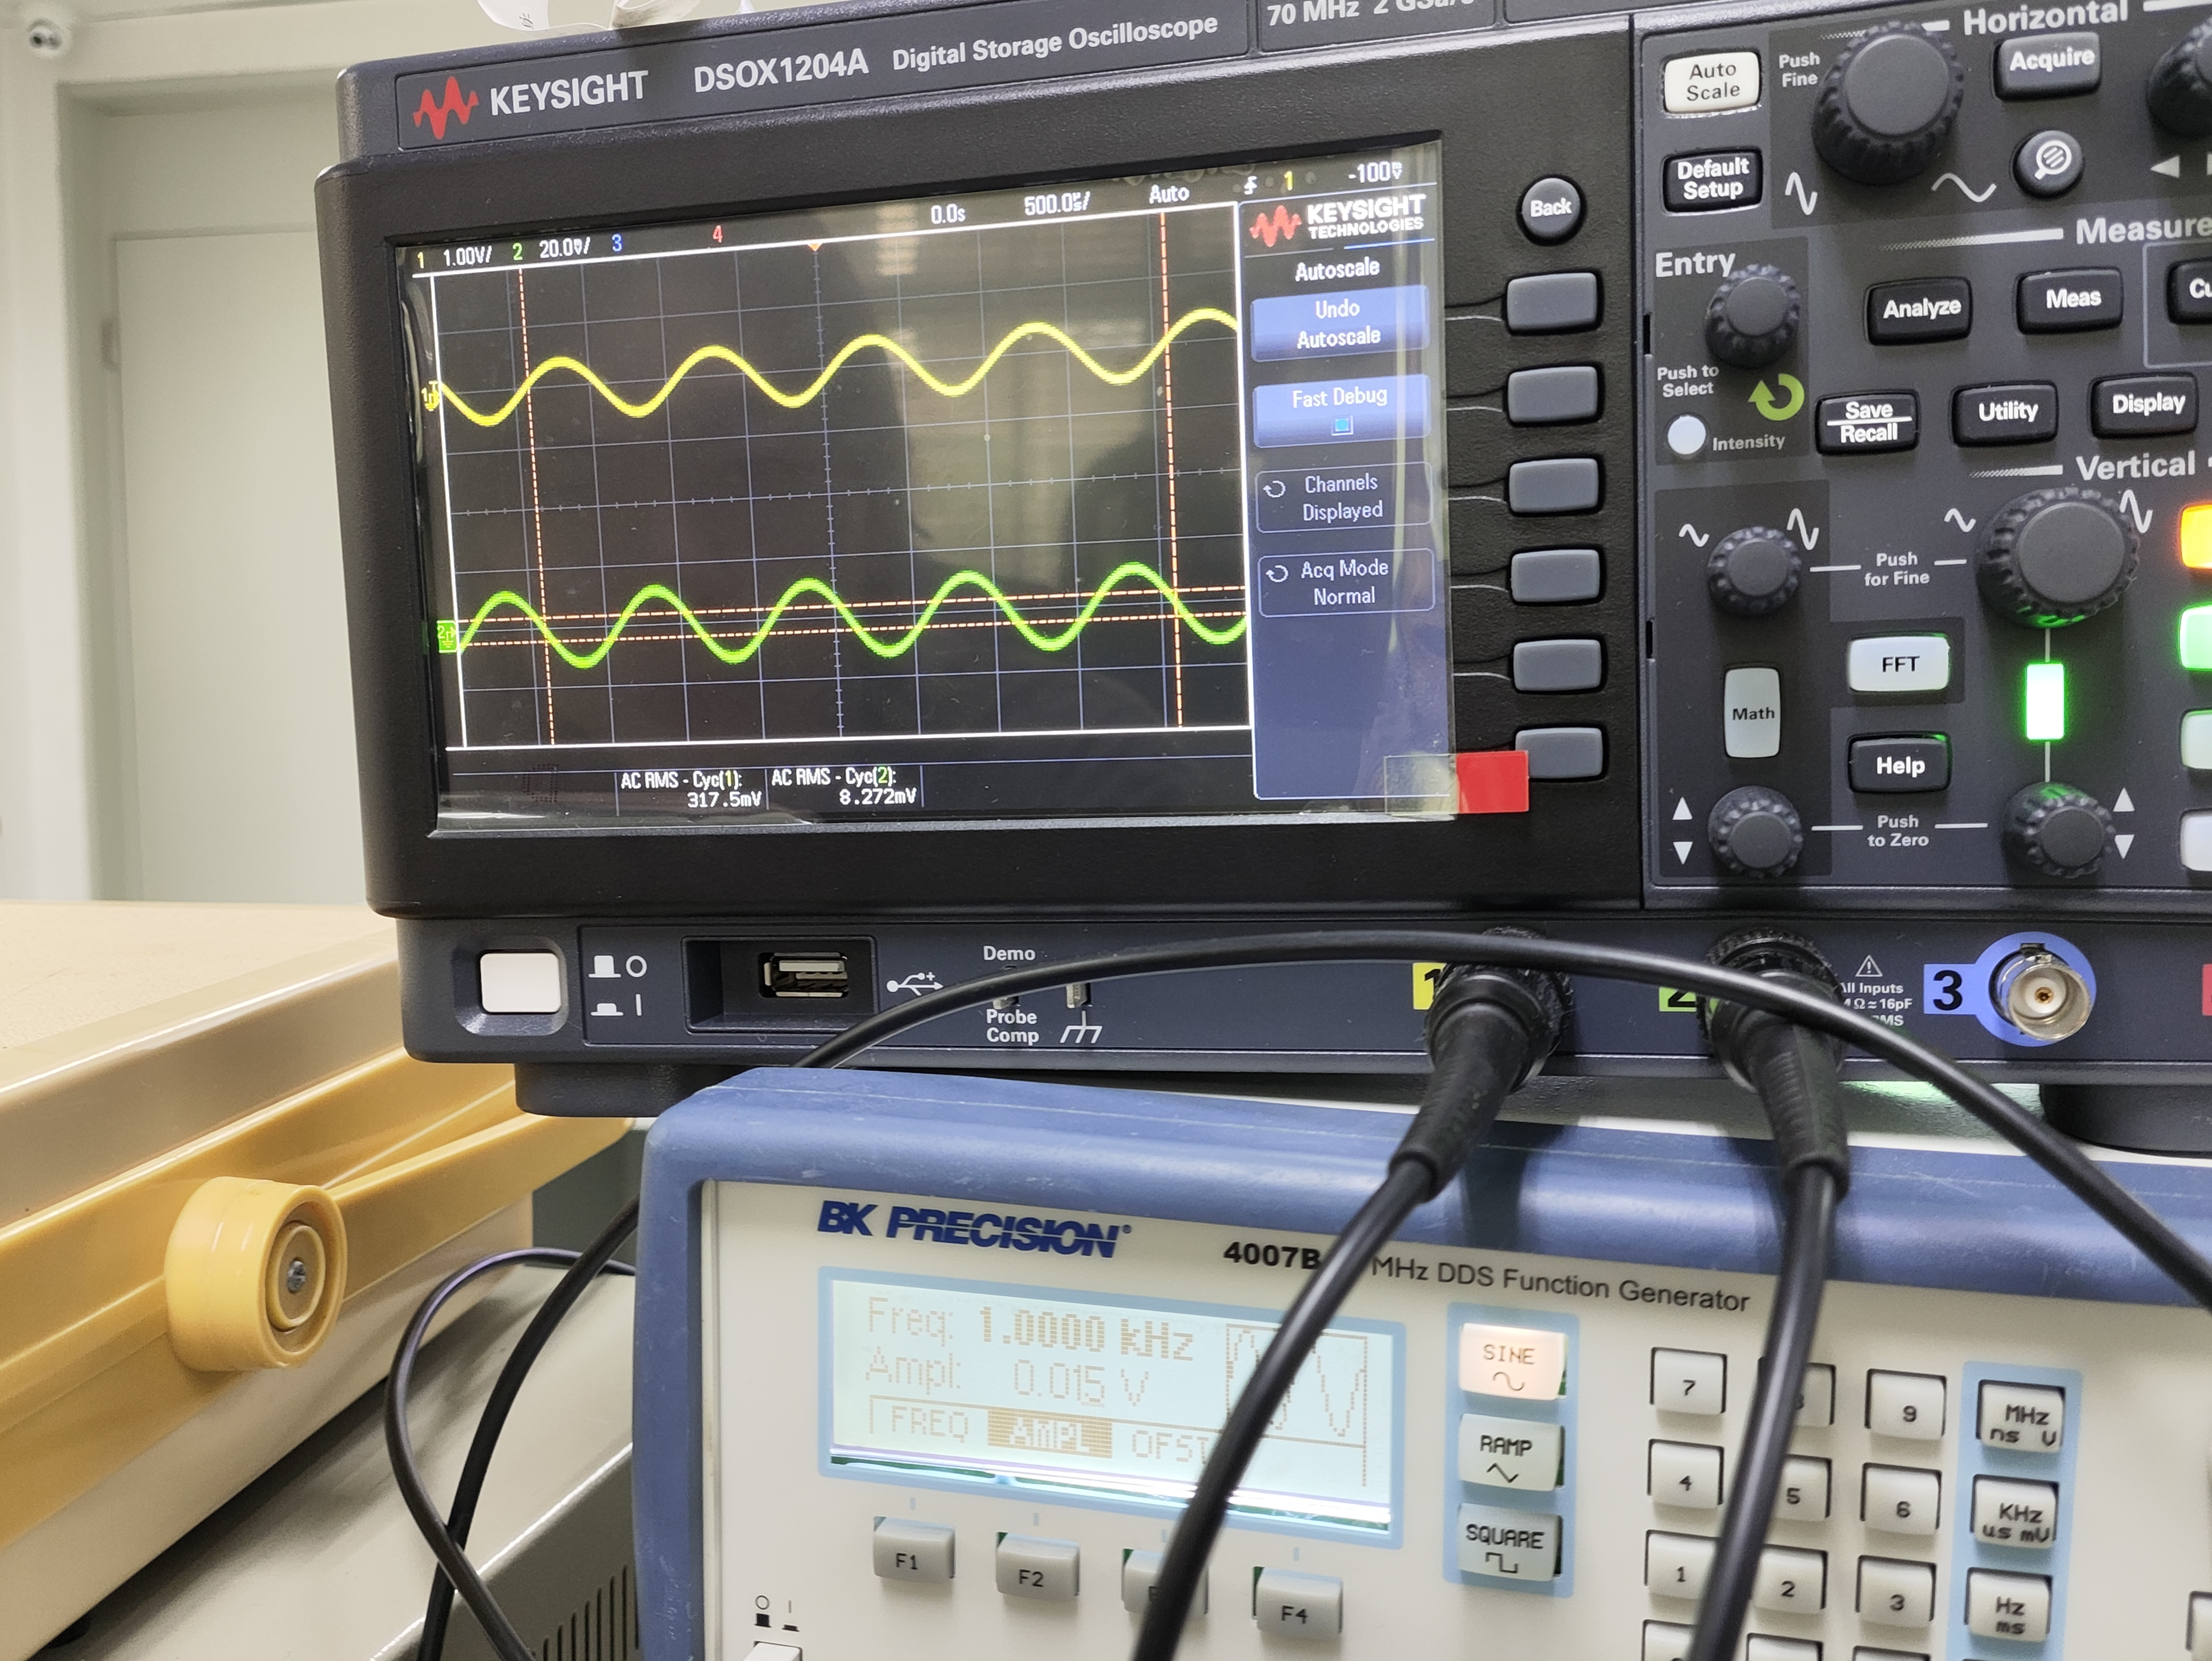
\includegraphics[width=1\linewidth]{Experiment_06/Images/6.5_Vo-Vib_015mV.jpg}
            \caption{0.015V Waveform}
            \label{l6acvg015}
        \end{subfigure}
        \begin{subfigure}{0.25\textwidth}
            \centering
            \includegraphics[width=1\linewidth]{Experiment_06/Images/6.5_Vo-Vib_010mV.jpg}
            \caption{0.10V Waveform}
            \label{l6acvg010}
        \end{subfigure}
    \end{figure}

    Finally, we can find the input and output impedence of the circuit by using the following equations:
    ($V^*$ = 0.025 V for Input, $V^*$ = 0.160 V for Output)\par
    \begin{table}[H]
    \centering
        \begin{tabular}{l|c}
        \hline
        $v_i=18.1mV$ & $V_{ib}=13.7mV$ \\
        $v_i=10.8mV$ & $V_{ib}= 8.2mV$  \\
        $v_i=7.24mV$ & $V_{ib}=5.48mV$ \\
        \end{tabular}
        \caption{Various Input voltage and $V_{ib}$}
    \end{table}
    From this, we can calculate the input impedence, which is 
    \begin{equation}
        R_i = 13.55k \Omega
    \end{equation}

    \begin{table}[H]
        \centering
            \begin{tabular}{l|c}
            \hline
            $R_L$ & $V_O$ \\
            $300k \Omega$ & $0.219V$ \\
            $2k \Omega$ & $0.393V$ \\
            \end{tabular}
        \end{table}
    From this, we can calculate the output impedence, which is
    \begin{equation}
        R_o = 0.982k \Omega
    \end{equation}
\subsection{Experiment Conclusion}
    \subsubsection{Conclusion}
    In this experiment, we have successfully measured the quiescent-point of a common-emitter BJT amplifier and evaluated the small-signal amplification function of a common-emitter amplifier. We have also calculated the input and output impedence of the circuit.